%27/02 - Raúl Guantes
\chapter{Redes biológicas y modelos de redes reguladoras}
\section{Redes complejas en biología}
Históricamente, las primeras redes que se caracterizaron al completo fueron la red del factor de transcripción de \textit{Escherichia coli} y las redes de interacción proteica en \textit{Saccharomyces cerevisiae}. Actualmente hay muchas bases de datos con las redes de muchos organismos. También hay redes neuronales de C. elegans. 

Las redes biológicas pueden representarse como «grafos» con nodos y conexiones. Cada nodo representa un elemento de la red, y las conexiones representan las interacciones entre los elementos.
Por ejemplo, la red de interacción de proteínas tiene un nodo para cada proteína y conexiones entre las proteínas que interaccionan entre sí. 

Analizando la estructura de la red y las conexiones entre los nodos podemos extraer algunas conclusiones sobre algunos «principios de diseño» biológicos:
\begin{itemize}
\item \textbf{Redes aleatorias:} las conexiones son equiprobables y aleatorias entre los nodos.
\item \textbf{Redes libres de escala:} hay unos ciertos nodos con más probabilidad de conexión que otros y que se denominan hubs. 
\item \textbf{Redes jerárquicas}
\end{itemize}

Las redes modernas en biología son:
\begin{itemize}
\item \textbf{Redes dinámicas o de evolución temporal}: las conexiones varían en el tiempo. Por ejemplo, la expresión de genes en una célula depende de perturbaciones. Los nodos se mantienen, pero son las conexiones las que van cambiando. 
\item \textbf{Redes multicapa:} hay diferentes tipos de redes que pueden interaccionar entre sí. Un ejemplo: en ecología hay muchas redes multicapa si se analizan las interacciones de virus y huéspedes. Una capa puede ser todos los tipos de virus, otra los tipos de plantas o huéspedes, otra con los distintos ambientes, etc. Otro ejemplo es una red de interacción de proteínas del virus con las proteínas del huésped. Las redes tienen distintas estructuras, dando lugar a un cierto tipo de dinámica entre esa red.
\item \textbf{Redes neuronales multiescala:} un ejemplo es la red neuronal que salió a finales de 2024 con la reconstrucción del cerebro completo de una mosca adulta. 
\end{itemize}

Para extraer información de las redes, primero se puede mirar la estructura que tiene. Una forma de ver si tiene una estructura especial es comparar la red con una aleatoria. Para el mismo número de nodos y conexiones, se reconecta la red al azar con equiprobabilidad. En la red real, se pueden describir hubs que están más conectadas. 

En biología, las redes suelen ser libres de escala y modulares. Estas redes son más robustas, es decir, si se elimina un nodo, la estructura no se perturba tanto o no colapsa. A esto se le conoce como \textbf{principio de robustez}.

\begin{figure}[h]
\centering
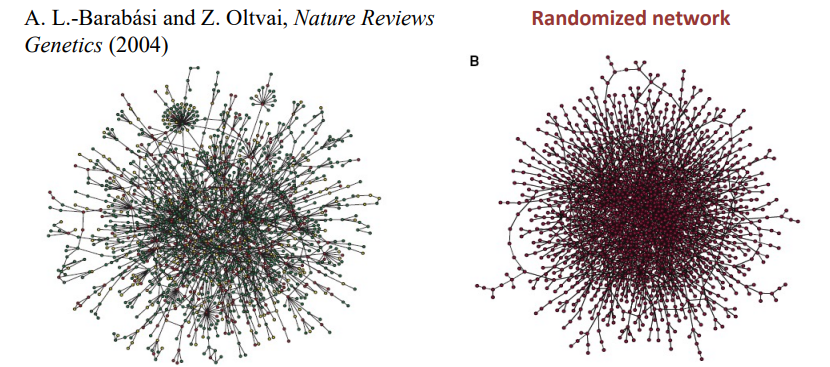
\includegraphics[width = 0.7\textwidth]{figs/biological-network.png}
\end{figure}

\section{Modularidad: motivos de redes}
Cuando se empezaron a estudiar las redes biológicas, se empezó a ver que la estructura de redes biológicas cambia la idea de la evolución de los sistemas biológicos. Como dijo François Jacob, 
\begin{quotation}
La naturaleza funciona por integración. Cualquiera que sea el nivel, los objetos analizados por las ciencias naturales son siempre organizaciones, o sistemas. Cada sistema de un nivel determinado utiliza como ingredientes algunos sistemas del nivel más simple, pero sólo algunos.
\end{quotation}

Algunos patrones dentro de una red compleja aparecen con mucha más frecuencia que otros (principio de recurrencia). Estos patrones se denominan \textbf{motivos o módulos de red}.

\begin{figure}[h]
\centering
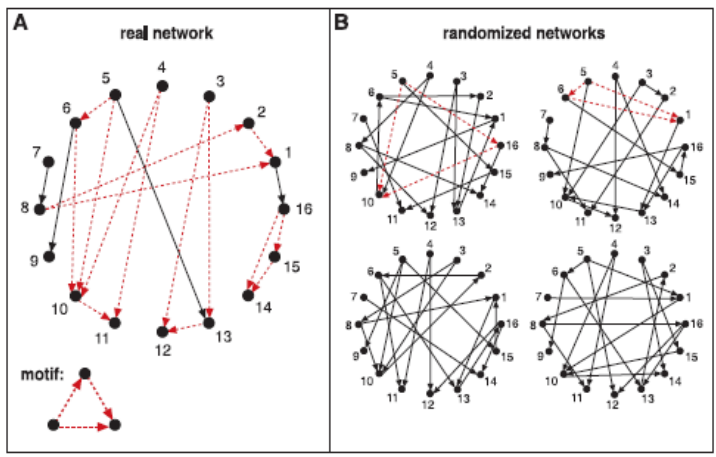
\includegraphics[width = 0.7\textwidth]{figs/motivo-redes.png}
\end{figure}

¿Los motivos de red representan entidades funcionales útiles? La biología de sistemas intentaba comprender la red biológica mediante representaciones más sencillas. 

\section{Redes de regulación transcriptómica}
En una red reguladora, los «nodos» son factores de transcripción. La actividad de cada gen viene dada por el nivel de proteína producida en un momento dado. 

La siguiente red fue construida en 2008 para representar todos los factores de transcripción que participan en el desarrollo embrionario humano. Mirando en detalle las conexiones entre los factores de transcripción, hay muchos motivos de retroalimentación: un nodo afecta a un segundo nodo, el cual a su vez afecta al primero, y cada uno de ellos tiene su propia retroalimentación. 

\begin{figure}[h]
\centering
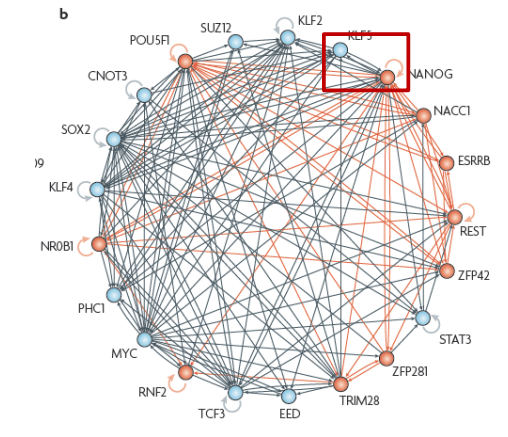
\includegraphics[width = 0.7\textwidth]{figs/red-embrionaria.png}
\end{figure}

La dinámica simple de nacimiento/muerte de una proteína Y que estudiamos (producción constante y degradación lineal) puede representarse mediante las reacciones bioquímicas: 
$$\frac{dY}{dt} = \alpha - \delta Y$$
Esto se considera en el modelo de la siguiente forma:
\begin{figure}[h]
\centering
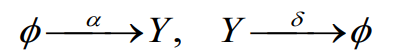
\includegraphics[width = 0.7\textwidth]{figs/reacciones.png}
\caption{Las proteínas Y se crean mediante $\alpha$, y desaparecen mediante $\delta$.}
\end{figure}

Algunas proteínas actúan como factores de transcipción, activando o reprimiendo la expresión de otra proteína. 

¿Cuánta proteína Y se produce en función de la cantidad de X que hay?
\begin{figure}[h]
\centering
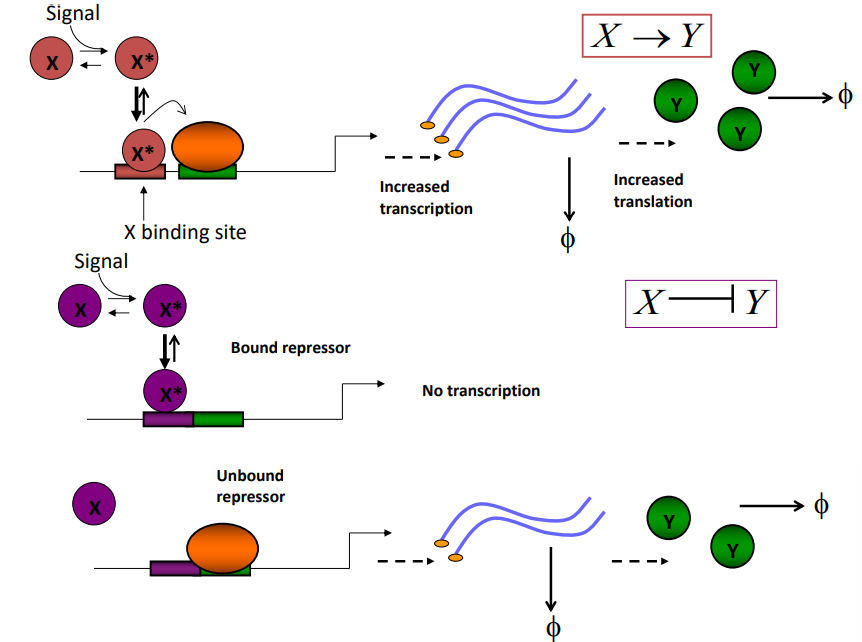
\includegraphics[width = 0.7\textwidth]{figs/factores-transcripcion.png}
\caption{Las proteínas activas se marcan con un asterisco. Cuando X es un activador, al unirse se favorece la transcripción de Y, aumentando su cantidad. Cuando X es un inhibidor, al unirse al gen no se produce la transcripción (no se genera Y).}
\end{figure}

Vamos a analizar esto de forma matemática.
\begin{enumerate}
\item \textbf{Escribir todas las especies (variables) de interés y las reacciones bioquímicas en las que interviene cada especie:}
\begin{itemize}
\item X: factor de transcripción inactivo
\item X*: factor de transcripción activo
\item P: promotor del gen Y libre
\item PX*: promotor del gen Y unido a X*
\item M: mRNA
\item Y: proteína resultante
\end{itemize}
Normalmente los factores de transcripción son activos cuando forman oligómeros (dos o más moléculas de X se asocian formando un complejo).

\item \textbf{Analizar las distintas reacciones o interacciones entre las variables:}
\begin{enumerate}
\item Activación / desactivación del factor de transcripción X. Esto se puede hacer por fosforilación o formación de complejos (oligómeros). 
$$nX \xrightarrow{K_a} X_n$$
$$X_n \xrightarrow{K_d} nX$$
siendo $K_a$ la constante de asociación y $K_d$ la constante de disociación.

\item Unión y desunión del factor de transcripción X al promotor P.
$$P + X_n \xrightarrow{K_b} (PX_n)$$
$$(PX_n) \xrightarrow{K_u} P + X_n$$
siendo $K_b$ la constante de unión (binding) y $K_u$ la constante de unbinding. 

\item Transcripción

Si es del promotor libre, da lugar al mRNA con una constante de transcripción $\beta$. Esto se da por ejemplo cuando X es un inhibidor y no está unido.
$$P \xrightarrow{\beta} P + M$$

Si X es un activador y está unido, la reacción se describe con la tasa de transcripción $\rho$:
$$(PX_n) \xrightarrow{\rho} (PX_n) + M$$

Si $\beta$ es mayor que $\rho$, X es un represor al haber más expresión si el factor de transcripción no está ligado. Si $\beta$ es menor que $\rho$, X es un activador, aumentando la expresión de la proteína tras la unión de X. 

\item Traducción
$$M \xrightarrow{\alpha} M + Y$$

\item Degradación de ARNm y proteínas con su velocidad de degradación $\delta$.
$$M \xrightarrow{\delta_M} \varnothing$$
$$Y \xrightarrow{\delta_Y} \varnothing$$
\end{enumerate}

\item \textbf{Considerar restricciones o ligaduras}
Una relación entre variables obvia es que, si la célula no se está dividiendo, el gen sólo puede estar en dos estados: libre u ocupado, por lo que su número de copias es constante.
$$P + PX_n = P^T (constante)$$

\item \textbf{Escribir la evolución temporal de cada especie utilizando la ley de acción de masas}
Ley de acción de masas dice que las velocidades de reacción son proporcionales a los productos de las concentraciones de reactivos.
La ecuación de ganancia/pérdida se describe como $dx/dt = production - degradation$. 

\begin{equation}
\tag{a}
\frac{dX}{dt} = nK_d \cdot X_n - nK_a \cdot X^n
\end{equation}
\begin{equation}
\tag{a,b}
\frac{dX_n}{dt} = K_a \cdot X^n + K_u \cdot (PX_n) - K_d \cdot X_n - K_b \cdot P \cdot X_n
\end{equation}
\begin{equation}
\tag{b}
\frac{dP}{dt} = K_u \cdot (PX_n) - K_b \cdot P \cdot X_n
\end{equation}
\begin{equation}
\tag{c}
\frac{d(PX_n)}{dt} = K_b \cdot P \cdot X_n - K_u \cdot (PX_n)
\end{equation}
\begin{equation}
\tag{c,e}
\frac{dM}{dt} = \beta P + \rho (PX_n) - \delta_M M
\end{equation}
\begin{equation}
\tag{d,e}
\frac{dY}{dt} = \alpha M - \delta_Y Y
\end{equation}

\item \textbf{Considerar las escalas temporales de las diferentes reacciones}
El problema de las constantes es que no se conocen. Una aproximación para simplificar las constantes es mediante agrupación de escalas temporales. La activación de un factor de transcripción tarda un milisegundo, y la unión de dicho factor a su sitio del ADN un segundo. Estos son reacciones rápidas. Por el contrario, la transcripción y traducción de un gen dura 5 minutos, y la degradación proteica dura hasta 1 hora, siendo reacciones lentas. Así, suponemos que las reacciones rápidas están en equilibrio con respecto a las lentas, y no las consideramos como variables dinámicas.
$$\frac{dX}{dt} = nK_dX_n - nK_aX^n \cong 0 \rightarrow \frac{X_n}{X^n} = \frac{K_a}{K_d} \equiv K_{act}$$
Definir de este modo las constantes de equilibrio para todas las reacciones rápidas permite eliminar variables. Por ejemplo, se puede expresar $X_n$ como:
$$X_n = K_{act} X^n$$
y, del equilibrio de unión y desunión al promotor, la variable del promotor ocupado se puede definir como:
$$(PX_n) =  \frac{K_b}{K_u} \cdot P \cdot X_n = K_{bind} \cdot P \cdot X_n = K_{bind} k_{act} P \cdot X^n = K_x P \cdot X^n$$
El último paso consiste en expresar la variable promotora libre P, que es una variable rápida, en función de la cantidad del factor de transcripción X. Utilizando la restricción $P + (PX_n) = 1$, obtenemos:
$$P + (PX_n) = 1 = P(1 + K_xX^n) \rightarrow P = \frac{1}{1 + K_xX_n}$$
De esta forma, eliminamos las ecuaciones para las variables rápidas, manteniendo sólo la dinámica del ARNm y de las proteínas, y expresando todas las variables rápidas en estas ecuaciones restantes como una función de X:
$$\frac{dY}{dt} = \alpha M - \delta_Y Y$$
$$\frac{dM}{dt} = \beta \frac{1}{1 + K_xX^n} + \rho \frac{K_xX^n}{1 + K_x X^n} - \delta_M M$$

Si asumimos que la transcripción de Y solo es posible cuando el factor de transcripción está unido:
$$\frac{dM}{dt} = \rho \frac{X^n K_x}{1 + X^nK_x} - \delta_M M$$

\item \textbf{Suposición del estado cuasi estacionario para el ARNm}
Cuando la degradación del ARNm ocurre mucho más rápido que la degradación proteica ($\delta_M >> \delta_Y$), entonces se puede suponer que: 
$$\frac{dM}{dt} \approx 0 \rightarrow \frac{dY}{dt} = \sigma_{act} \frac{X^n K_x}{1 + X^n K_x} - \delta_Y Y$$

Así, podemos expresar cómo cambia la concentración de equilibrio de nuestra proteína Y en función de la cantidad de X (nuestra «entrada») en términos de una función de Hill (también llamada función de respuesta, función de regulación o relación entrada/salida):
$$f(x) = \frac{(X/\theta)^n}{1 + (X/\theta)^n}$$

\begin{figure}[h]
\centering
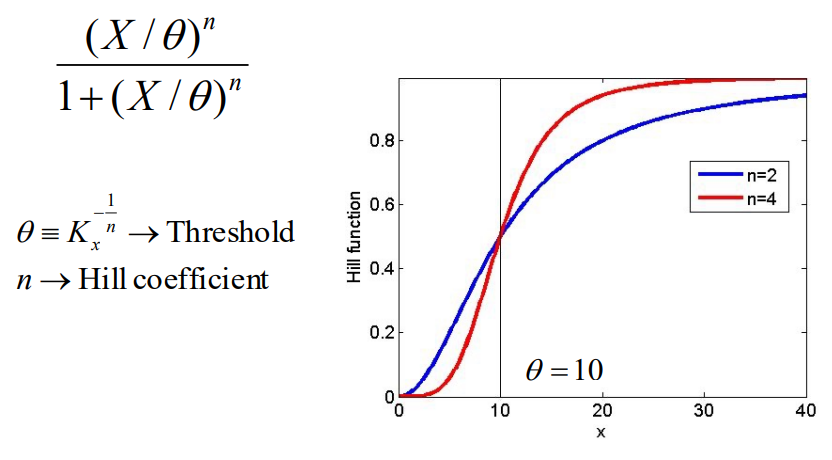
\includegraphics[width = 0.6\textwidth]{figs/hill-function.png}
\end{figure}
Para $n \rightarrow \infty$, se produce una función escalón. En este caso, n representa la cooperatividad, el número de oligomerización o fosforilaciones necesarias para que funcione. Proporciona la pendiente de la subida. $\theta$ representa el umbral de producción.

Si asumimos que la transcripción del gen Y solo se puede dar cuando el promotor está libre, entonces
$$\frac{dY}{dt} = \sigma_{rep} \frac{1}{1 + X^n K_x} - \delta_Y Y$$
y se representa en la función represora de Hill.

\begin{figure}[h]
\centering
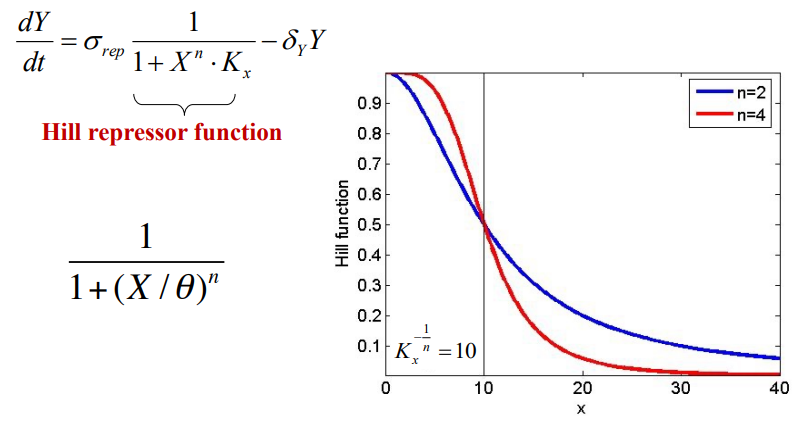
\includegraphics[width = 0.6\textwidth]{figs/hill-function-rep.png}
\end{figure}

En resumen, las interacciones entre genes pueden cuantificarse mediante funciones sigmoidales (Hill) con dos parámetros (umbral de activación/represión y cooperatividad).
\end{enumerate}

Puede haber casos donde haya varios reguladores para una proteína, siendo esto muy frecuente en eucariotas. Cuando hay varios inputs que están activando al mismo nodo, puede haber muchas combinaciones posibles del efecto de esos inputs. 

\begin{figure}[h]
\centering
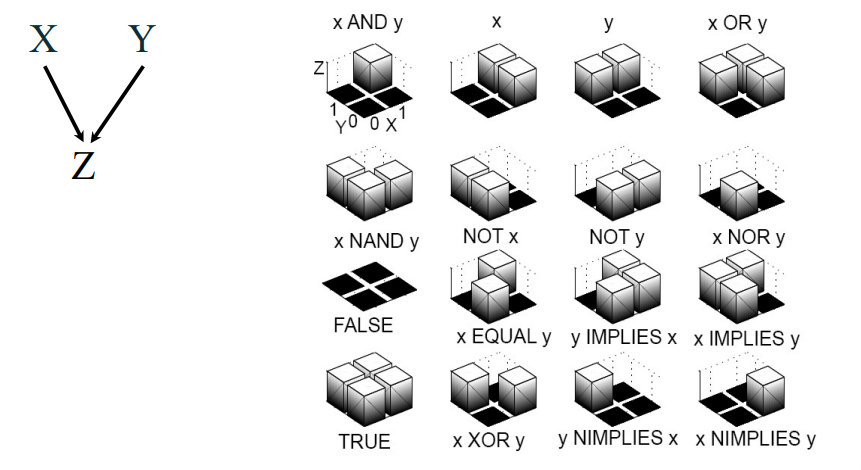
\includegraphics[width = 0.8\textwidth]{figs/logic-gates.png}
\end{figure}

Una puerta de tipo AND se puede representar de la siguiente forma:
$$f(x,y) = \frac{(X/K_x)^n}{1 + (X/K_x)^n} \times \frac{(Y/K_y)^n}{1 + (Y/K_y)^n}$$

En el caso de una puerta OR:
$$f(x,y) = \frac{(X/K_x)^n}{1 + (X/K_x)^n} + \frac{(Y/K_y)^n}{1 + (Y/K_y)^n}$$

\section{Función de motivos de redes en redes reguladoras}
Los bucles de retroalimentación se dan cuando hay una interacción de X a Y y de Y a X. Para ver cómo es la retroalimentación, se debe multiplicar el efecto de todas las interacciones (ver si un bucle es positivo o negativo).

Se distinguen los feedforward loops (FFL) coherentes, donde una interacción y otra tienen el mismo efecto, de los FFL incoherentes donde hay efectos contrarios.

\subsection{Motivo de red más simple: autorregulación}
El motivo de red más simple es el de un gen autoregulado, ya sea de forma positiva o negativa. En \textit{E. coli}, hay 400 nodos y 500 enlaces. Por azar, esperaríamos que hubiese 1,2 autorfegulaciones (500/400). Como se trata de una distribución independiente de Poisson, realmente es de $1.2 \pm \sqrt{1.2}$. De forma experimental, se encontraron 40 autorregulaciones negativas, siendo esto mucho mayor de lo esperado.

Suponemos que hay un gen que produce la proteína Y a partir de una señal con velocidad $\alpha$ y se degrada en $\delta$. 
$$\frac{dY}{dt} = \alpha - \delta Y$$

¿Cuál es el tiempo de respuesta a la señal? El tiempo de respuesta se considera que es la mitad del valor estacionario $\alpha/\delta$. Como la función se describe con la fórmula
$$Y(t) = \frac{\alpha}{\delta} (1 - e^{-\delta t})$$
el tiempo de respuesta se calcularía de la siguiente forma:
$$Y(t-T_{resp}): \frac{\alpha}{2 \delta} = \frac{\alpha}{\delta} (1 - e^{-\delta T_{resp})}$$
teniendo que despejar $T_{resp}$.

%06/03 - Raúl Guantes
El tiempo de respuesta de un gen es el tiempo necesario para llegar a la mitad de la respuesta total:
$$T_{1/2} = \frac{\ln 2}{\delta}$$
Si la proteína es estable y sólo se degrada por dilución, entonces $T_{1/2} = T_{div}$. Esto es un proceso muy lento. Para poder aumentar su velocidad, se podría aumentar $\delta$, teniendo que aumentar por consiguiente también $\alpha$. 

\subsubsection{Autorregulación negativa}
Considerando un gen con autorregulación negativa, cambia en el tiempo con el término
$$\frac{dY}{dt} = f(Y) - \delta Y$$
siendo $f(Y)$ la tasa de producción y $\delta Y$ la tasa de degradación. Como es una autorregulación negativa, $f(Y)$ tendrá la forma de una sigmoidal negativa (por ejemplo, $f(Y) = \frac{1}{1 + (Y/k)^2}$. El valor de equilibrio se dará cuando $f(Y) = \delta Y$. La gráfica que define esto se denomina como gráfica del balance de tasas o rate balance plot:
\begin{figure}[h]
\centering
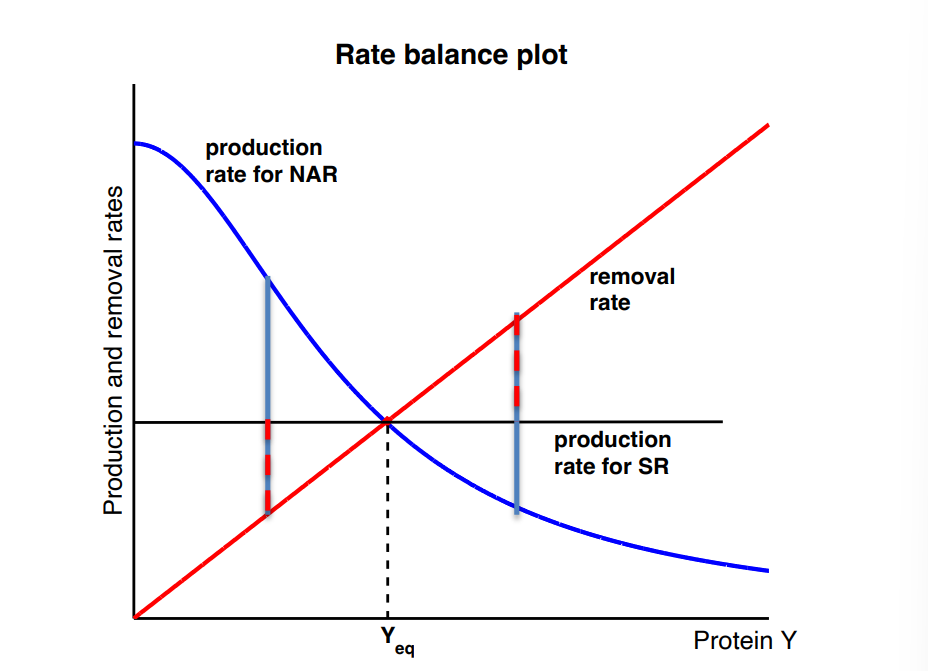
\includegraphics[width = 0.6\textwidth]{figs/rate-balance-plot.png}
\end{figure}

Al calcular la derivada, se vería que ese punto de equilibrio sería estable, el cual depende del umbral de represión $Y/k$ que biológicamente depende de la afinidad de la proteína por el promotor. El tiempo de respuesta depende de la magnitud de la derivada; cuanto mayor sea en valor absoluto, mayor velocidad de cambio.

Para un modelo sin regulación (producción constante):
$$\frac{dY}{dt} = \alpha - \delta Y$$
Para comparar los tiempos de respuesta, se debe comparar el valor absoluto de la derivada.
\begin{itemize}
\item $Y < Y_{eq}$: la tasa de cambio de la autorregulación negativa es más grande que la tasa de cambio de la regulación simple.
\item $Y > Y_{eq}$: el valor absoluto de la tasa de cambio de la autorregulación negativa es mayor que el valor absoluto de la tasa de cambio de la regulación simple. 
\end{itemize}

La autorregulación negativa acelera el tiempo de respuesta.
\begin{figure}[h]
\centering
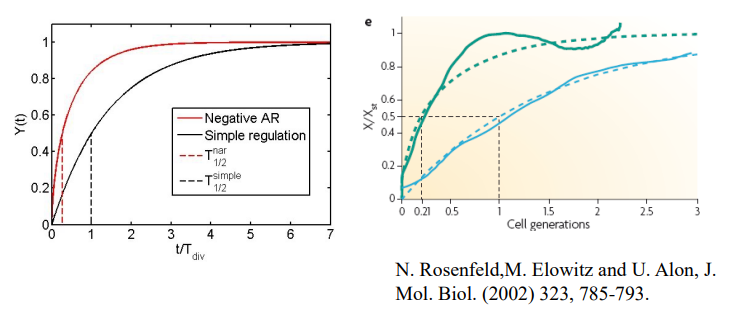
\includegraphics[width = 0.8\textwidth]{figs/nar.png}
\end{figure}

\subsubsection{Autorregulación positiva}
Para una autorregulación positiva, la proteína se describe con la misma función:
$$\frac{dY}{dt} = f(Y) - \delta Y$$
Ahora, $f(Y)$ es creciente con forma de función de Hills, mientras que la tasa de degradación sigue con una forma de recta. El punto en el que se cortan es el punto de equilibrio, el cual es estable. En este caso, el valor absoluto de la derivada del modelo sin regulación es mayor que el valor de la derivada del modelo con autorregulación positiva. Por tanto, la autorregulación positiva aumenta el tiempo de respuesta (es más lento). 
\begin{figure}[h]
\centering
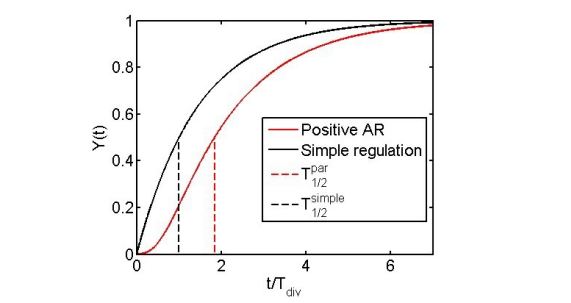
\includegraphics[width = 0.8\textwidth]{figs/par.png}
\end{figure}

Tanto la producción como el ciclo celular tienen fluctuaciones, por lo que necesita genes que respondan más rápido y más lentamente. Si $\delta$ cambia, la función de degradación cambia, teniendo mayor o menor pendiente. Cuando hay producción constante, el valor de equilibrio se mueve, mientras que la tasa de producción con autorregulación negativa apenas se ve modificada. Por tanto, la autorregulación negativa produce resistencia frente a fluctuaciones en producción $\alpha$ o en tiempos de división $\delta$. 

Si la función de autorregulación más suave ($f(Y) = \frac{(Y/k)^n}{1 + (Y/k)^n}$), entonces habrá más puntos de equilibrio. El punto de equilibrio en 0 es estable, al igual que aquel en el que la producción de proteína se satura. Entre ellos, debe haber un punto de equilibrio inestable, el cual separa las condiciones iniciales. Por tanto, tenemos un modelo de biestabilidad con dos estados posibles: $Y_{eq} = 0, Y_{eq}^{max}$. Todo esto se produce si $f(Y)$ es cooperativo. 

Poniendo un ejemplo concreto, suponemos que $n = 2$ y que $k = 1$. Por tanto, el modelo que tenemos es:
$$\frac{dY}{dt} = s + \frac{Y^2}{1 + Y^2} - \delta Y$$
siendo $s$ las señales bioquímicas. 

Si no hay señales bioquímicas ($s=0$), los puntos de equilibrio se deben calcular de la siguiente forma:
$$Y \frac{Y}{1 + Y^2} = \delta Y \begin{cases}
Y^1_{eq} = 0 \\
\frac{Y}{1 + Y^2} = \delta
\end{cases}
$$
$$\delta Y^2_{eq} + \delta - Y_{eq} = 0$$
$$Y_{eq} = \frac{1 \pm \sqrt{1 - 4 \delta^2}}{2}$$
$$1 - 4 \delta^2 > 0 $$
$$4 \delta^2 < 1$$
$$\delta < 1/2$$

Por tanto, hay tres puntos de equilibrio, los cuales causan la bifurcación silla-nodo. 

Añadiendo un inductor ($s$), la recta de degradación se desplaza hacia los lados desde el origen. Para un $\delta = 0.55$ y $s=0$, no hay producción. No obstante, cuando $s = 0.2$, la producción basal aumenta la producción de la proteína, viéndose amplificada por la autorregulación positiva. Esto se conoce como \textbf{interruptor genético}.  

\begin{figure}[h]
\centering
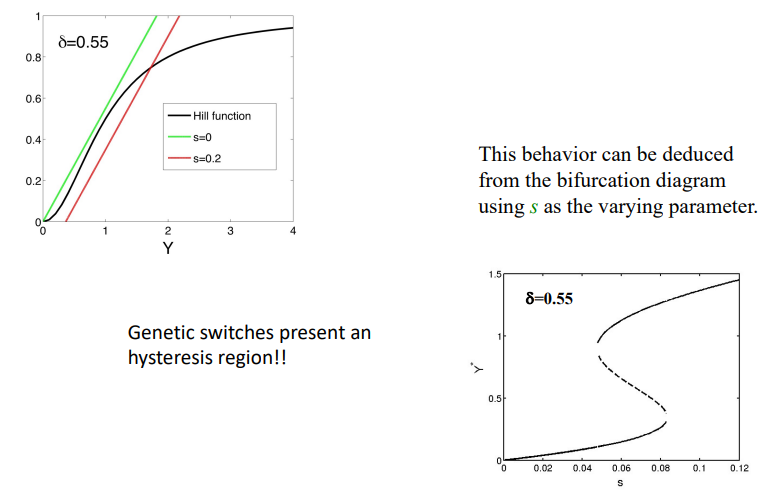
\includegraphics[width = \textwidth]{figs/genetic-switch.png}
\end{figure}

Si pintamos los puntos de equilibrio en valor del parámetro $s$, vemos que se produce una región de histéresis. 

Cuando hay interacciones mutuas con una variable y dos autorregulaciones positivas o negativas, hay más estados posibles: que se expresen los dos, ninguno o solo uno de ellos. En la activación mutua, si ambos son 0, no hay activación. Si con una señal se produce un poco de x, aumenta, activando y, llegando un momento en el que los dos pasan a estar expresados de forma máxima ($(0,0) \rightarrow (1,1)$). Si después se quita la señal, los estados siguen aumentados, no disminuyen debido a la histéresis. Un estímulo transitorio se convierte así en una respuesta permanente, a lo que se llama memoria celular. En una inhibición mutua, si un gen está expresado, el otro se reprime: $(0,1) \rightarrow (1,0)$
\begin{figure}[h]
\centering
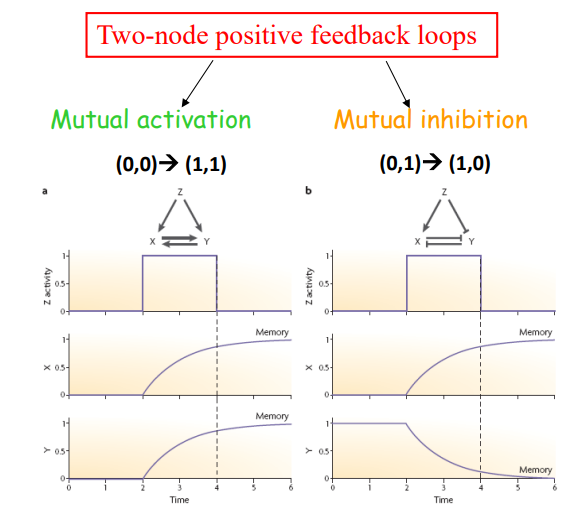
\includegraphics[width = 0.6\textwidth]{figs/cellular-memory.png}
\end{figure}

Si se combinan las retroalimentaciones positivas y negativas, se pueden dar los cuatro estados: $(0,0), (0,1), (1,0), (1,1)$. Esto se ha demostrado útil en la diferenciación de células madre.

\begin{figure}[h]
\centering
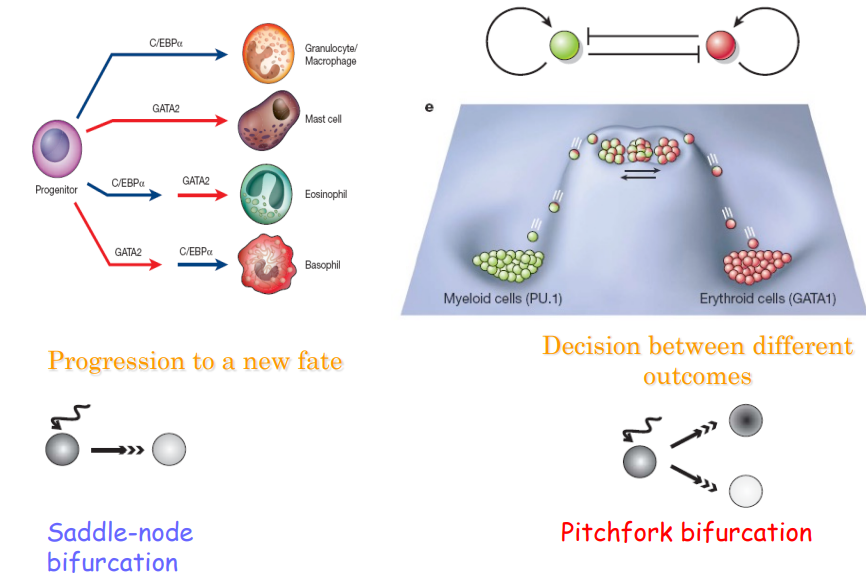
\includegraphics[width = 0.8\textwidth]{figs/stem-differentiation.png}
\end{figure}

Se puede representar un paisaje epigenético que describe los valles y colinas con los distintos destinos celulares. Las redes de regulación celulares dan lugar a que se enciendan o apaguen distintos genes en distintos estados. 

\begin{figure}[h]
\centering
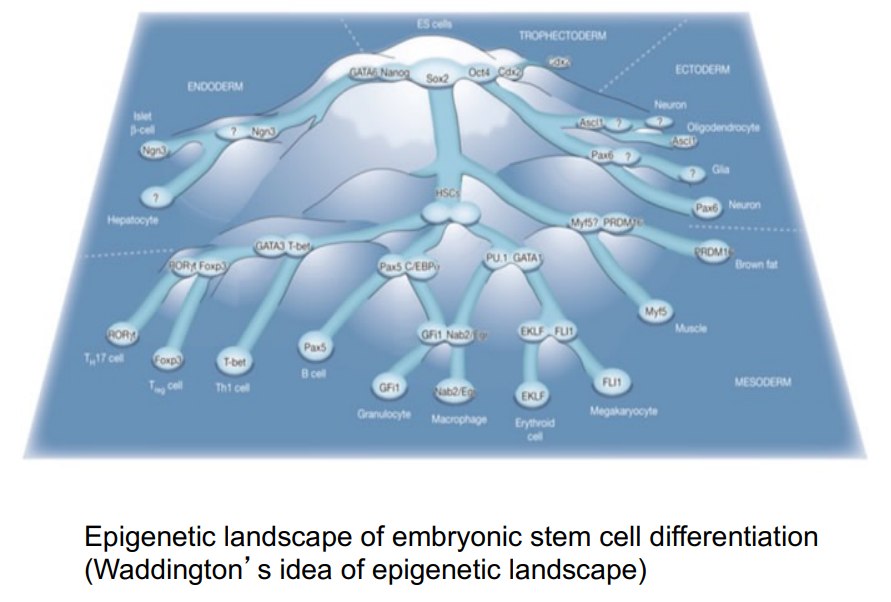
\includegraphics[width = 0.8\textwidth]{figs/waddington.png}
\end{figure}

\subsection{Feedback negativo y oscilaciones}
Hay muchos procesos fisiológicos y de señalización celular regulados por ritmos periódicos y oscilaciones. Los ritmos circadianos son comunes a muchos organismos, tanto mamíferos como bacterias o levaduras. La información está codificada en la frecuencia y el número de pulsos, como puede ser la activación de genes selectivos por factores de transcripción, señalización de calcio, respuesta a estrés, etc. En todos los ejemplos se han identificado proteínas o reguladores que interaccionan con las proteínas fundamentales de las respuestas mediante un feedback negativo. 

\begin{figure}[h]
\centering
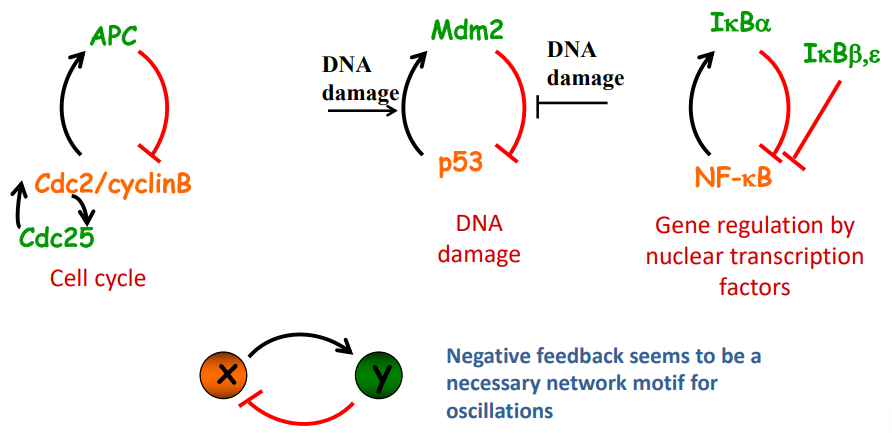
\includegraphics[width = 0.8\textwidth]{figs/feedback-negativo.png}
\end{figure}

Suponiendo que tenemos dos proteínas que interaccionan mediante un feedback negativo: una favorece a otra, la cual inhibe a la primera. Los mecanismos por los que un modelo dinámico oscila de forma robusta son los ciclos límite. Todos los ejemplos que tienen oscilaciones son debidos a los ciclos límite. Las condiciones para que haya un ciclo límite es la existencia de un punto inestable en el centro, el cual se denomina como espiral inestable. El tipo de bifurcación en el que una espiral estable pasa a inestable se conoce como bifurcación de Hopf, la cual implica la creación de un ciclo límite. Las espirales son autovalores complejos de la matriz jacobiana. Para un sistema de dos variables, hay una función $f(y)$ y una función $g(x)$, siendo la matriz jacobiana la matriz con las derivadas de las funciones en el punto de equilibrio. Los autovalores se pueden oner como la traza de las dos variables. Para tener bifurcación Hopf, el determinante debe ser positivo y la parte real debe pasar por 0, lo que equivale a que la traza pase por 0. 

Suponemos dos genes con interacciones mutuas. La producción de x depende de y. Suponemos que el término de degradación es $\delta x,y$.
$$\frac{dx}{dt} = f(y) - \delta x$$
$$\frac{dy}{dt} = g(x) - \delta y$$

La matriz jacobiana sería de la siguiente forma:
$$\vec{J} = \begin{pmatrix}
- \delta & \frac{\sigma f}{\sigma y} \\
\frac{\sigma g}{\sigma x} & - \delta
\end{pmatrix} \rightarrow \begin{pmatrix}
\text{Efecto de X sobre X} & \text{Efecto de Y sobre X} \\
\text{Efecto de X sobre Y} & \text{Efecto de Y sobre Y}
\end{pmatrix}$$
Así, la traza siempre va a ser negativa ($-2 \delta$). La matriz debe tener la siguiente estructura:
$$\vec{J} = \begin{pmatrix}
+ & + \\
- & -
\end{pmatrix}$$
o
$$\vec{J} = \begin{pmatrix}
+ & - \\
+ & -
\end{pmatrix}$$

Los elementos de las dos diagonales deben tener signos distintos para que pueda aparecer un ciclo límite. Para conseguir un signo positivo en la diagonal es mediante la autorregulación positiva de x o de y. El jacobiano representa el efecto de cada una de las variables sobre ellas mismas (en la diagonal) o sobre la otra (no diagonal).

\begin{figure}[h]
\centering
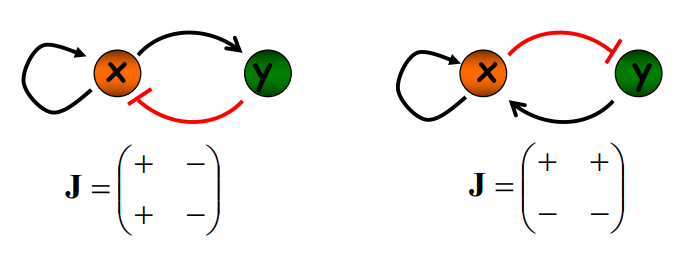
\includegraphics[width = 0.8\textwidth]{figs/feedback-jacobiano.png}
\end{figure}

Sin feedback negativo, no habría determinante positivo y, por tanto, ciclo límite. Se necesita feedback negativo, pero con autorregulación positiva. El signo positivo de la diagonal implica una autorregulación positiva, mientras que el signo negativo no implica autorregulación negativa, si no que hay degradación y no hay autorregulación. 

Por lo tanto, para que existan oscilaciones en redes de dos componentes, en principio son necesarias tanto la retroalimentación negativa como la autorregulación positiva (un ejemplo es el oscilador del ciclo celular). En el caso del modelo Lotka-Volterra, la autorregulación positiva sería la tasa de crecimiento por reproducción, mientras que la retroalimentación negativa es la interacción presa-predador. 

El feedback positivo no es estrictamente necesario, ya que el feedback negativo produce un desfase temporal entre las interacciones que ya produce las oscilaciones. El motivo de retroalimentación negativa más simple, la autorregulación negativa, puede mostrar oscilaciones si se introduce explícitamente un retraso en la transcripción y traducción del gen.

El retraso en el módulo combinado de retroalimentación negativa con autorregulación positiva viene dado por el bucle de retroalimentación positiva que ralentiza las respuestas.

\begin{figure}[h]
\centering
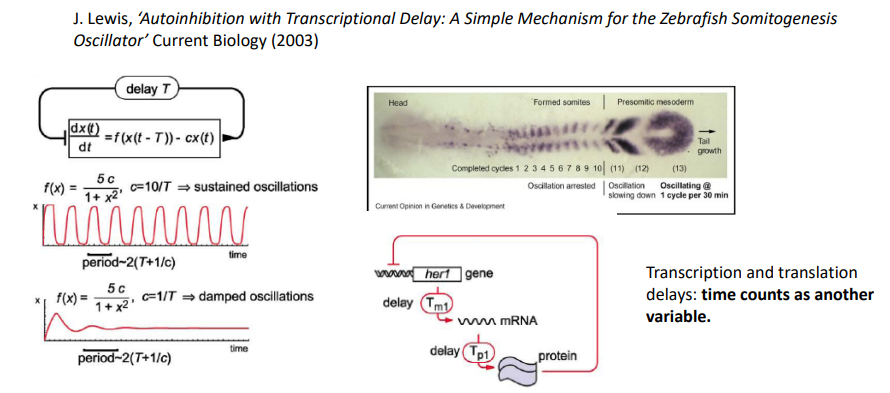
\includegraphics[width = 0.8\textwidth]{figs/autoinhibition-delay.png}
\end{figure}

Los osciladores con retroalimentaciones negativas y positivas entrelazadas aparecen con más frecuencia en los sistemas biológicos debido al principio de robustez: El periodo y la amplitud de las oscilaciones no deben variar tanto con el ruido molecular. El oscilador con retroalimentación positiva es mucho más robusto frente a las fluctuaciones naturales en la abundancia de los componentes. 